\documentclass[12pt]{article}
\usepackage{amsmath}
\usepackage{graphicx}
\usepackage{hyperref}
\usepackage[utf8]{inputenc}
\usepackage[spanish]{babel}
\usepackage[margin=3cm]{geometry}
\usepackage{amsfonts}
\usepackage{listings}
\usepackage[T1]{fontenc}
\usepackage{float}
\usepackage{subfig}
\usepackage{pdfpages}
\usepackage{times}
\usepackage{tikz}
\usetikzlibrary{matrix}

\colorlet{helpful}{lime!70}
\colorlet{harmful}{red!30}
\colorlet{internal}{yellow!20}
\colorlet{external}{cyan!30}
\colorlet{F}{helpful!50!internal}
\colorlet{D}{harmful!50!internal}
\colorlet{O}{helpful!50!external}
\colorlet{A}{harmful!50!external}

\newcommand{\texta}{Útiles}
\newcommand{\textb}{Peligrosos}
\newcommand{\textcn}{Análisis interno}
\newcommand{\textdn}{Análisis externo}
\newcommand{\back}[1]{\fontsize{100}{110}\selectfont #1}

\title{Emprendimiento y Transferencia de Conocimiento.}
\author{Néstor Rodríguez Vico. DNI: 75573052C - \href{mailto:nrv23@correo.ugr.es}{nrv23@correo.ugr.es}}
\date{\today}

\makeatletter
\def\@seccntformat#1{%
	\expandafter\ifx\csname c@#1\endcsname\c@section\else
	\csname the#1\endcsname\quad
	\fi}
\makeatother


\lstdefinestyle{bash_style}{
	language=bash,
	frame=single,
	xleftmargin=.25in,
	upquote = true,
	basicstyle=\scriptsize,
	breakatwhitespace=false,         
	breaklines=true,                 
	captionpos=b,                    
	keepspaces=true,                 
	numbers=left,                    
	numbersep=5pt,                  
	showspaces=false,                
	showstringspaces=false,
	showtabs=false,                  
	tabsize=2
}

\lstset{style=bash_style}

\begin{document}
\maketitle

\setlength{\belowdisplayskip}{5pt} 
\setlength{\belowdisplayshortskip}{5pt}
\setlength{\abovedisplayskip}{5pt} 
\setlength{\abovedisplayshortskip}{5pt}

\section{Introducción.}

En este documento encontramos la recopilación de los trabajos a aportar en la asginatura. Los trabajos realizados son:

\begin{itemize}
	\item Desarrollo de una propuesta sencilla de plan inicial (modelo de negocio) utilizando el método CANVAS + DAFO.
	\item Realización de una ficha de búsqueda de financiación empresarial.
	\item Ejercicio práctico de búsqueda de patentes.
	\item Realización en casa de un vídeo individual (``Elevator Pitch'' de menos de 5 minutos) grabado por cada estudiante, presentando su idea de negocio.
	\item Realización de una tabla con previsiones financieras.
	\item Ejercicio de desarrollo de creatividad y de liderazgo.
\end{itemize}

\section{Modelo de negocio.}

Mi idea de negocio surge tras una necesidad mía hace unos años. Tiempo atrás me enfrenté por primera vez al diseño de una página web. Mi primer problema fue aprender las sintáxis \textit{HTML} y la sintáxis \textit{CSS}. Una vez tenía una página web estática, tocaba darle ese toque visual que tanto cuesta conseguir, animaciones, colores, movimiento... Mi idea de negocio consiste en un sistema software que permite crear una páginas \textit{web} en tiempo real a partir de un boceto. \\

La primera etapa consiste en dibujar a mano alzada un primer boceto de como te gustaría que fuese tu página web y el sistema, usando técnicas de visión por computador, irá creando una página \textit{web} completamente funcional en tiempo real. A su vez, el sistema generará el boceto en versión digital para su posterior uso y modificación. Tras tener el primer diseño, podremos usar una interfaz gráfica del sistema para modificar la versión digitalizada para añadir animaciones y movimiento de una forma sencilla. Esto permite también una fácil actualización de la página \textit{web} en caso de que sea necesario. \\ 

Dicho sistemas será lo suficientemente modulas como para permitir añadir nuevas funcionalidades mediantes \textit{plugins} y extensiones. Por ejemplo, de partida, tendría un \textit{plugin} que permita generar la versión móvil y \textit{tablet} de la página \textit{web} a la vez que la versión de escritorio o un \textit{plugin} que permitirá subir la página \textit{web} a un servidor para que sea accesible por cualquier persona. \\

Un \textit{software} de este estilo permite a personas sin ningun conocimiento de programación tener una página \textit{web} funcional donde puedan publicirta su negocio de forma gratuita, fomentando así el crecimiento de los pequeños comercios. \\

A continuación muestro el método \textit{CANVAS} de mi idea de negocio:

\begin{figure}[H]
	\centering
	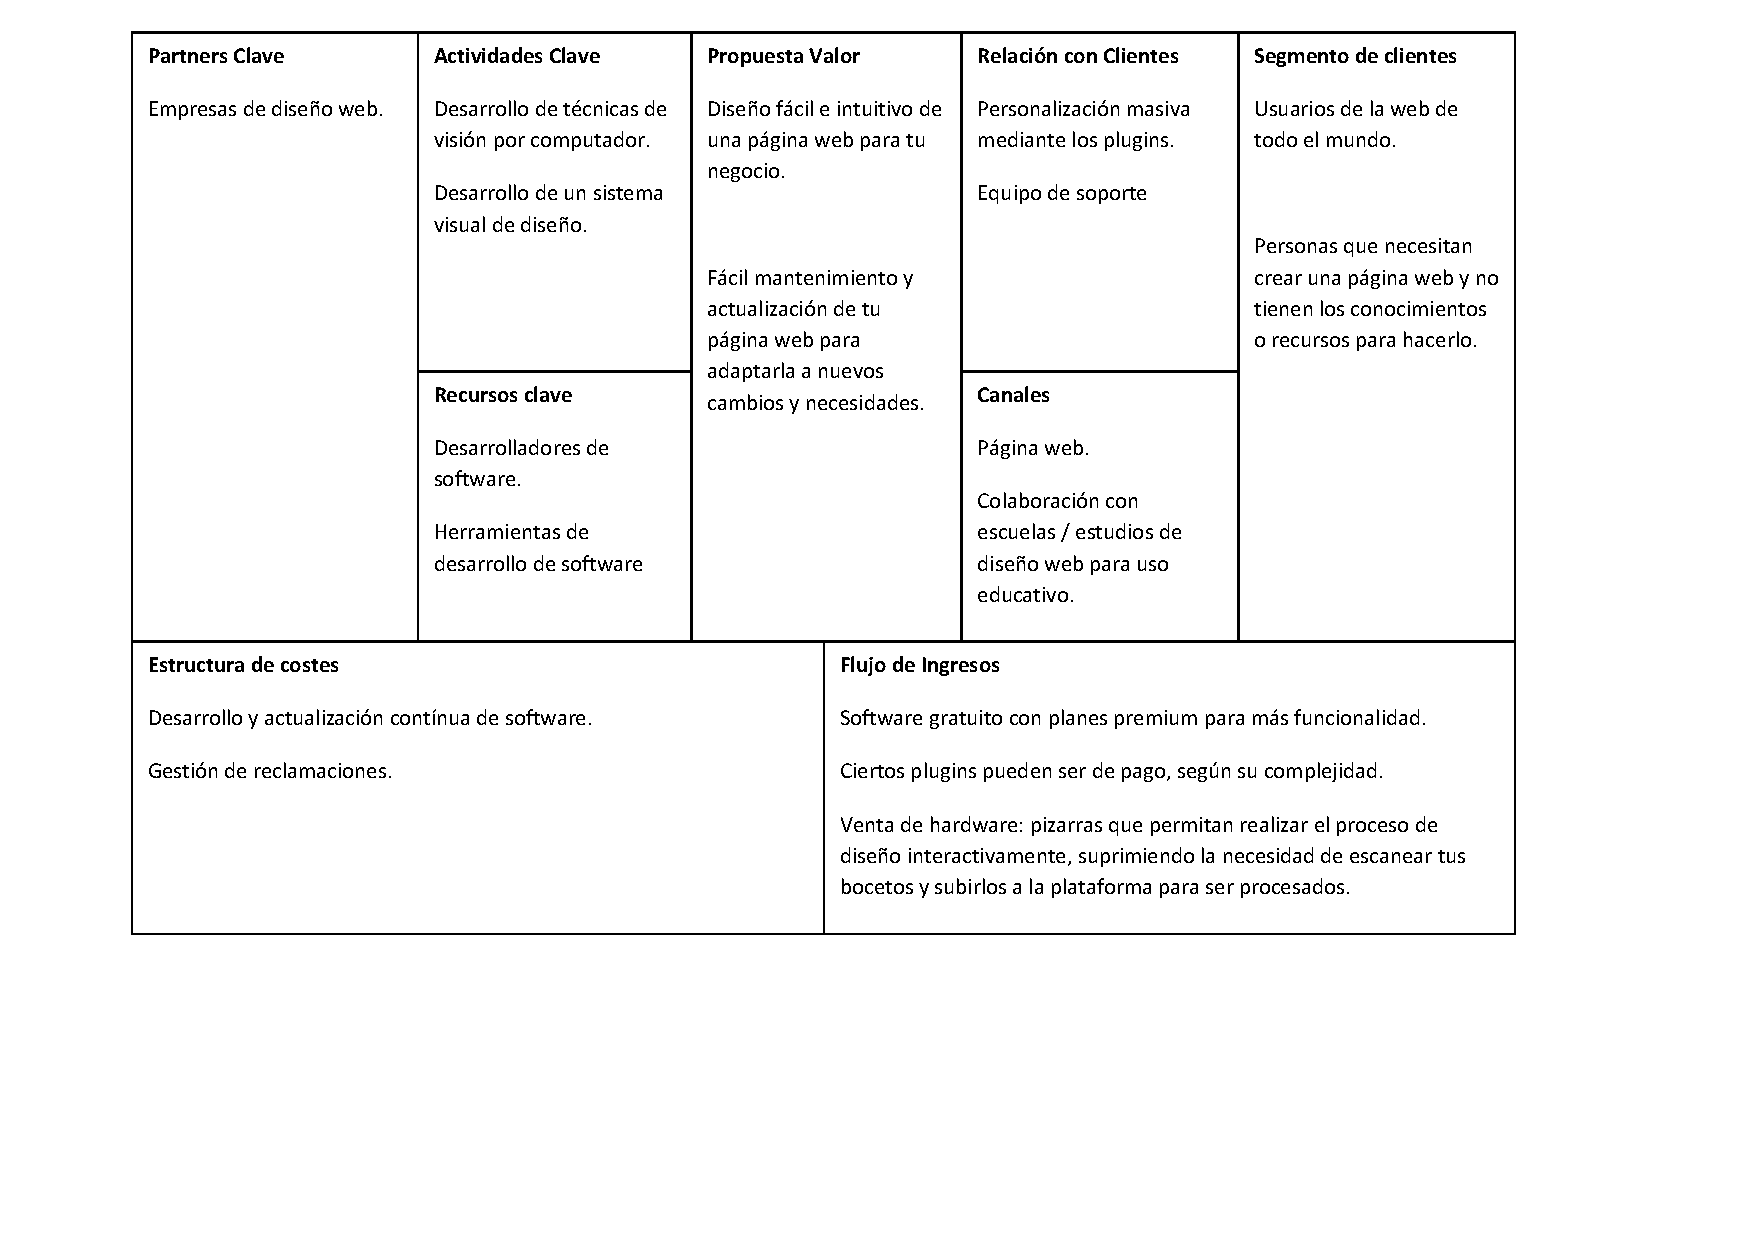
\includegraphics[width=\textwidth, trim={1.5cm 5cm 3.5cm 0.5cm}, clip]{canvas.pdf}
\end{figure}

A continuación muestro el método \textit{DAFO} de mi idea de negocio:

\begin{tikzpicture}[
    any/.style={minimum width=6cm,minimum height=6cm,%
                 text width=5.5cm,align=center,outer sep=0pt},
    header/.style={any,minimum height=1cm,fill=black!10},
    leftcol/.style={header,rotate=90},
    mycolor/.style={fill=#1, text=#1!95!black}
]

\matrix (SWOT) [matrix of nodes,nodes={any,anchor=center},%
                column sep=-\pgflinewidth,%
                row sep=-\pgflinewidth,%
                row 1/.style={nodes=header},%
                column 1/.style={nodes=leftcol},
                inner sep=0pt]
{
          &|[fill=helpful]| {\texta} & |[fill=harmful]| {\textb} \\
			|[fill=internal]| {\textcn} & |[mycolor=F]| \back{F} & |[mycolor=D]| \back{D} \\
			|[fill=external]| {\textdn} & |[mycolor=O]| \back{O} & |[mycolor=A]| \back{A} \\
};

\node[any, anchor=center] at (SWOT-2-2) {Sistema visual e intuitivo. \\ \vspace{0.15cm} Gratuito. \\ \vspace{0.15cm} Curva de aprendizaje rápida. \\ \vspace{0.15cm} Resultados en tiempo real.};
\node[any, anchor=center] at (SWOT-2-3) {Ausencia de ideas. \\ \vspace{0.15cm} Desconfianza por parte del usuario en hacerlo uno mismo. \\ \vspace{0.15cm} Entrar en un mercado establecido y maduro.};
\node[any, anchor=center] at (SWOT-3-2) {La gente está más familiarizada con la tecnología y muchos buscan la idea de promocionar su negocio mediante una página \textit{web}. \\ \vspace{0.15cm} Si no buscas una página \textit{web} muy compleja, puedes tenerla de forma gratuita, sin necesidad de contratar a un estudio de diseño \textit{web}.};
\node[any, anchor=center] at (SWOT-3-3) {Los usuarios potenciales pueden pensar que no tienen conocimientos suficientes y que no merece la pena ni intentarlo.\\ \vspace{0.15cm} Hoy en día es más fácil conocer a un amigo que sepa algo de informática y te pueda hacer una página \textit{web} básica sin tener que hacerlo tú.};
\end{tikzpicture}
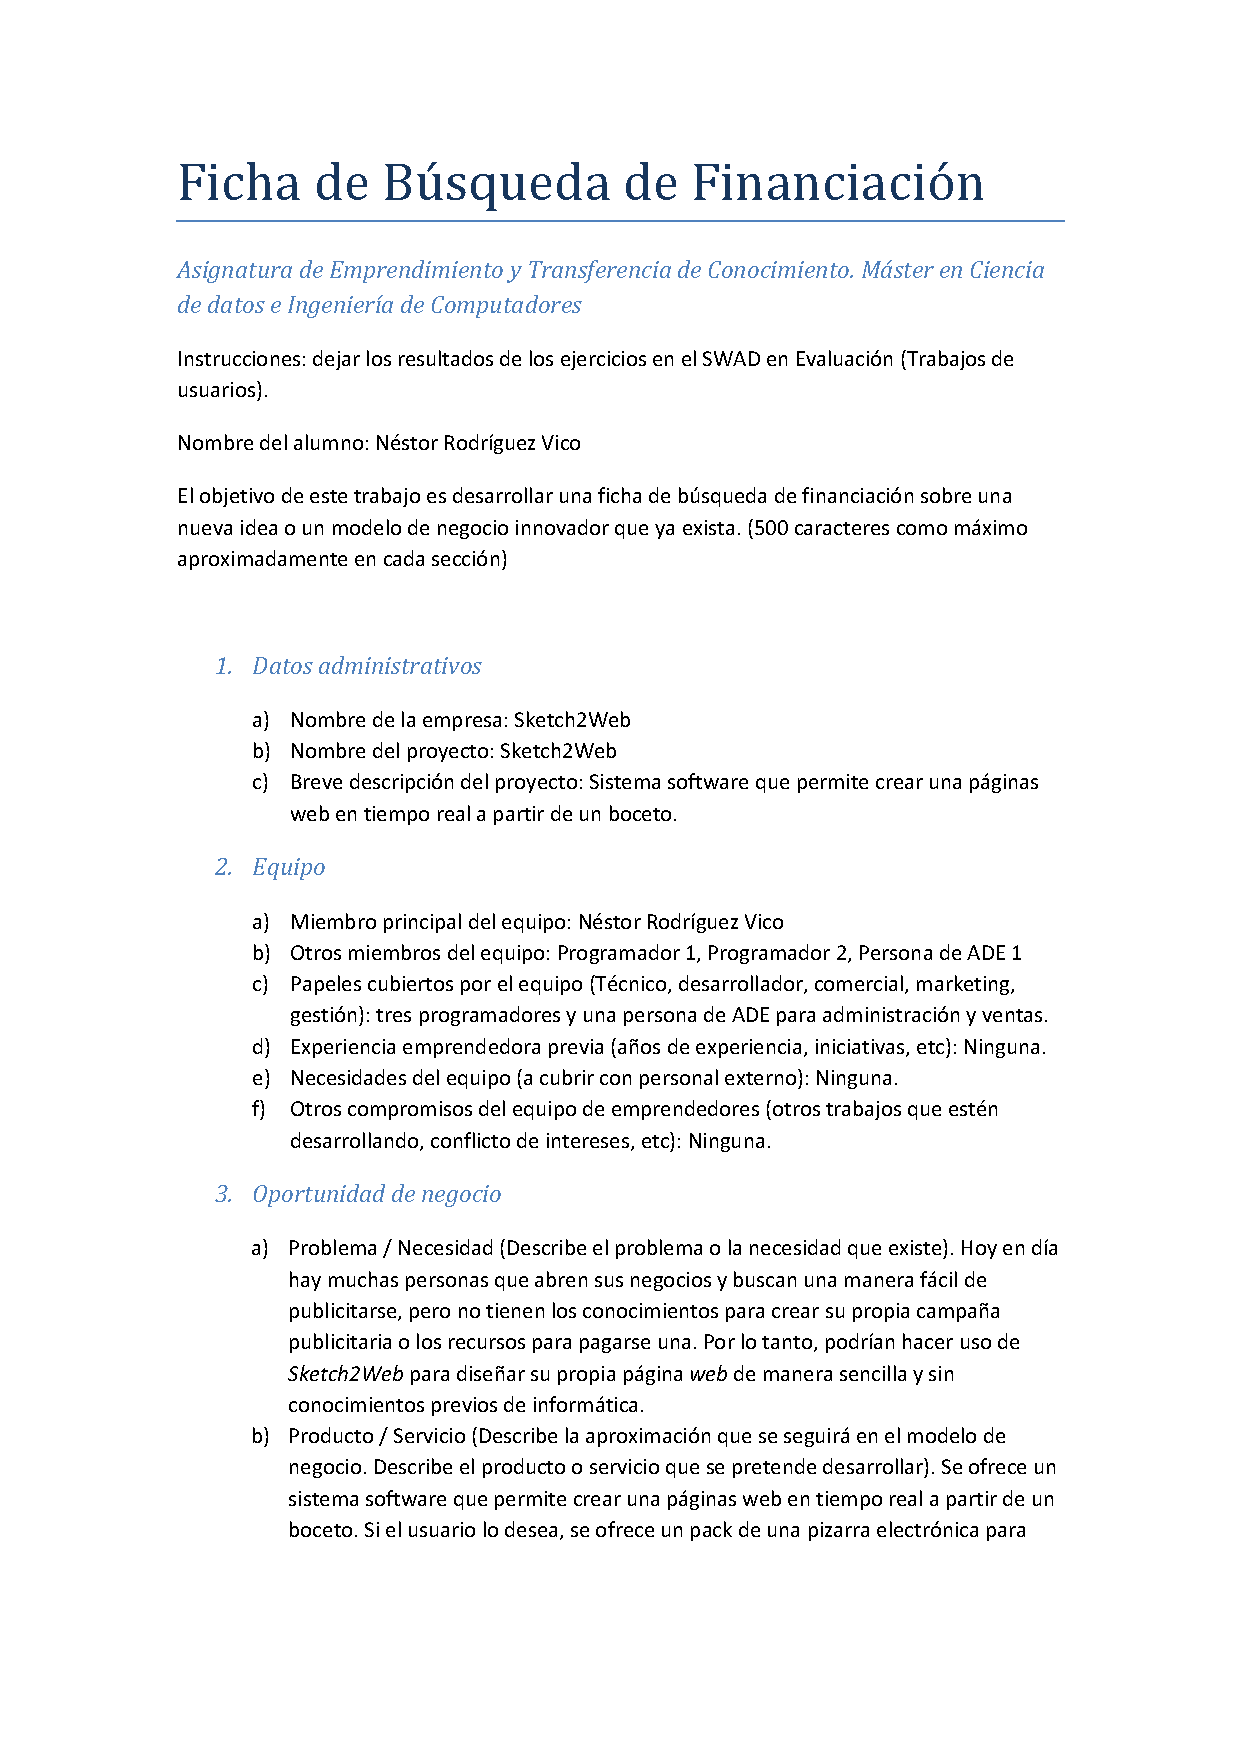
\includepdf[pages=-]{BusquedaFinanciacion.pdf}
\includepdf[pages=-]{patentes.pdf}

\section{Realización de una tabla con previsiones financieras.}

\textbf{Ejercicio 1.} \textit{Escribir dos ``tecnologías'', un sustantivo y un adjetivo (sencillos). Se escoge al azar uno de cada. Proponer un producto o servicio basándonos en la tupla.} \\

Para la generación las sustantivos y adeketivos aleatorios he usado la página desarrollada por Daniel Pinero \href{http://www.danielpinero.com/generador-palabra-aleatoria}{http://www.danielpinero.com/generador-palabra-aleatoria}. \\

Las tecnologías usadas han sido \textit{Servidores} y \textit{Java}. El adjetivo ha sido \textit{remoto} y el sustantivo \textit{notificación}. Con esta tupla podríamos pensar en desarrollar un software que nos permita centralizar todas las notificaciones recibidas y emitidas por nuestros servidores en un único lugar. Para ello, podríamos tener pequeños agentes \textit{Java} en cada servidor que deseamos monitorizar que se encargarían de redirigir dicha información a un servidor centralizado para que, en caso de haber una emergencia, tener que revisar sólo las alertas en dicho servidor y no en cada uno de los disponibles en nuestra infraestructura. \\

\textbf{Ejercicio 2.} \textit{De la lista de empresas fracasadas disponible en \href{https://www.cbinsights.com/blog/startup-failure-post-mortem/}{https://www.cbinsights.com/blog/startup-failure-post-mortem/}
seleccionen como mínimo una empresa (puede elegir más) y comente el porqué de su fracaso. Discusión ¿hay solapamientos o paralelismos?}

\begin{itemize}
	\item Título: \textit{We ran out of money}. Producto: \textit{Driver}. Razón: Driver compañía se encagaba de buscar emparejamientos para realizar ensayos clínicas. Dicha compañía cerró tras dos meses de funcionamiento. La razón del cierre fue la falta de dinero ya que no fueron capaces de conseguir fondos.
	
	\item Título: \textit{A Very Sad Goodbye}. Producto: \textit{OSSIC}. Razón: OSSIC era una empresa que surgió en \textit{Kickstarter} ofertando unos auriculares. La propia compañía admitió que su producto era ambicioso y costoso de desarrollar. Con los fondos de la campaña de crowdfunding la empresa pudo desarrollar las primera unidades, pero necesitaban más capital para poder producir los auriculares de forma masiva.
\end{itemize}

Como podemos ver, ambas empresas han cerrado por falta de capital. No he analizado más empresas con detalle en este documento, pero si leemos las razones por las que cierran las empresas en dicha página web, podemos ver que muchas de ellas cierran por falta de capital para desarrollar la actividad por la cual fueron creadas. \\

\textbf{Ejercicio 3.} \textit{Escriba una reflexión sobre cómo ha aplicado o echado en falta la aplicación de un liderazgo situacional en su vida profesional (académica en su defecto).} \\

En mi caso, voy a hablar de mi experiencia académica. Cuando surgen trabajos en grupo siempre hay alguién que asume el rol de líder y es el encargado de organizar y liderar el trabajo que se va a realizar. Muchas veces esta situación es favorable si se trata de un buen líder. Para mí, un buen líder es el que sabe motivar a su equipo, es capaz de organiar al equipo y hacerles ver que luchan/trabajan por un bien común. Los problemas vienen cuando el que se ha puesto de líder no es capaz de ver lo mejor para el equipo y lo que hace es elegir lo mejor para sus amigos en vez de para el grupo entero. Otro problema es cuando hay varias personas que quieren ser líderes y se producen confrontaciones entre ellos. En estas siatuaciones, puede ser que el equipo intente elegir a uno de ellos, lo cual conllevaría a más confrontaicones entre los apoyantes del otro líder, fragmentando aún más el equipo. 

\end{document}